\documentclass{beamer}
\usepackage{beamerthemeshadow}
\usepackage{graphicx}
\begin{document}
\title{COMP3111h Father-Focus project presentation}
\author{CHEN Lixi, LI Tao, ZHANG Yaofeng, ZHANG Zhijun}

\begin{frame}
\titlepage
\end{frame}
\begin{frame}\frametitle{Table of contents}\tableofcontents
\end{frame}


\section{Introduction}
\subsection{How the idea came up}
\begin{frame}\frametitle{Introduction}
\begin{itemize}
\item We are in a day of post-PC era
\item We have smartphones, and ...
\end{itemize}

\pause
\begin{figure}
 
\includegraphics[width=0.2\textwidth]{fb_log}
 \hspace{1cm}
 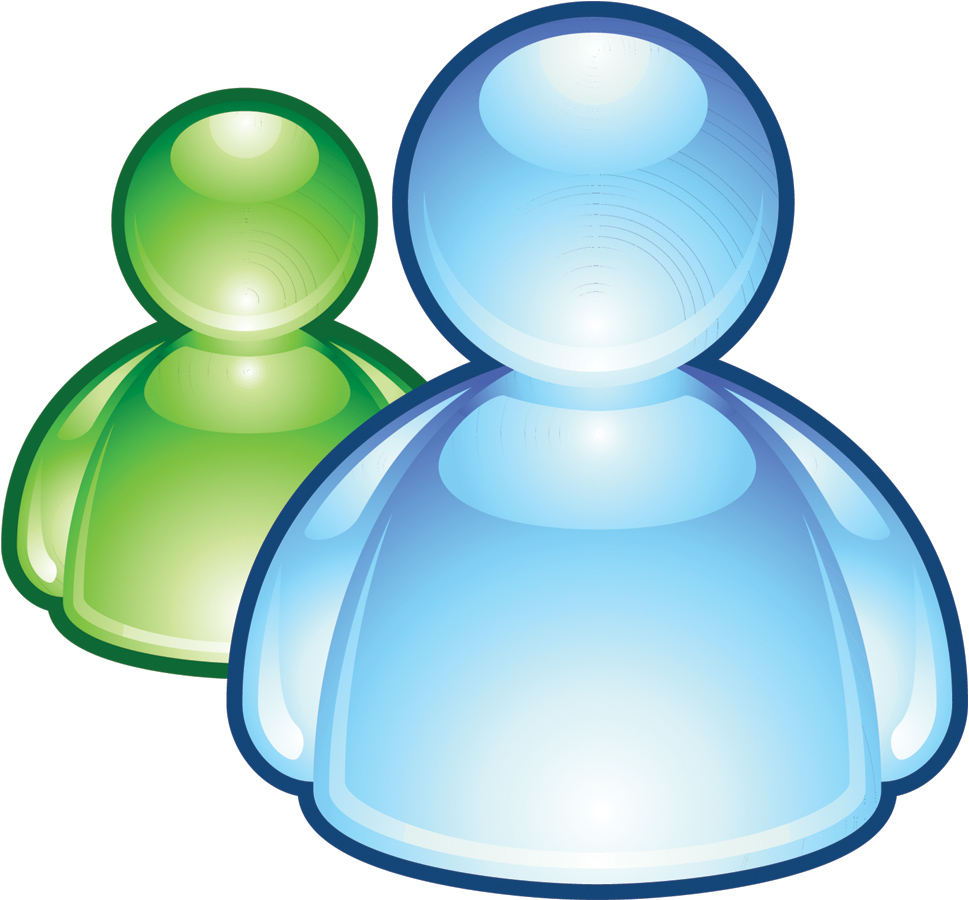
\includegraphics[width=0.2\textwidth]{MSN_logo}
 \hspace{1cm}
 
\includegraphics[width=0.2\textwidth]{tw_logo}
\end{figure}
...
\end{frame}

\begin{frame}
 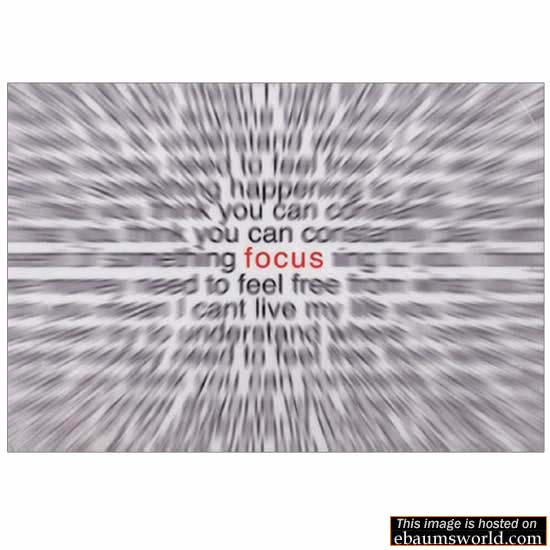
\includegraphics[width=0.95\textwidth]{focus}
\end{frame}

\subsection{Our goal}
\begin{frame}\frametitle{Our goal}
So our goal is to develop a application that:
\begin{itemize}
\item Help users manage and keep track on the tasks
\pause
\item Get users' lives organized and never missed a dealine with reminders, lists
and widgets. 
\pause
\item Most importantly, Reduce the distraction coaused by some application, keep
users \textbf{focus} on what you are doing.
\end{itemize}
\end{frame}
\subsection{Hightlights and innovation}
\begin{frame}\frametitle{Hightligths and innovation}
\begin{itemize}
\item Probably the first application to keep track on how much time you spent on
each project and give you statistics. 
\pause
\item The first application to limit application usage, and help user keep
focus.
\pause
\item  Access your tasks anywhere with automatic syncing accross phone and the
web server.
\pause
\item Easy to use and highly customized.
\end{itemize}

\end{frame}
\section{System Overview}
\subsection{Timer}
\begin{frame}\frametitle{Timer Activity}
Easily keep track on how much time you spent on each tasks:
\pause
\begin{itemize}
\item Easily slide to the task
\pause
\item Press start to start to timing.
\pause
\item The application will record the start time and the end time.
\pause
  \begin{itemize}
    \item For users to review the task, statistics will be generated
    \item If the time limited is setted, there will be a notification 
  \end{itemize}
\end{itemize}
\end{frame}

\subsection{System Locker}
\begin{frame}\frametitle{System Locker}
Keep you focus, just like your father:
\begin{itemize}
\item Take over the system locker when you are doing tasks, that is when the timer is going.
\pause
\item Make it cumbersome to unlock the system, by inputing a long string, or
even solve a difficult math problem. 
\pause
\item Interesting notification will be shown when you open a limited application
\pause
\item Like what your father do, increase the difficulty to distract.
\end{itemize}
\end{frame}

\subsection{Task Manager}
\begin{frame}\frametitle{Task Manager}
This is more than a to-do list manager! It carefully organize and categorize
your tasks, with kind notification!
\begin{itemize}
\item Add tasks easily: Task name is the only thing needed to create a task
\pause
\item Highly customized: You can add any information if you want, and
categorize it easily.
\pause
\item Kind reminder: You can specify the time and frequency to remind you or
just leave the work to the application, it will remind you
automatically based on the due day and importance you specify.
\pause
\item A chart will be generated to show the statistics for each tasks. Keep
trak how much time you spent for each task. Help you better arrange your time
and schedule. 
\pause
\item A personal assistant for you!
\end{itemize}
\end{frame}

\subsection{Data sync and web application}
\begin{frame}\frametitle{Database and sync}
Never loose your data:
\begin{itemize}
\item Sync the data with the cloud, never loose your tasks
\pause
\item Access your data anywhere with internet connection and browers.
\end{itemize}
\end{frame}


\subsection{Other functions}
\begin{frame}\frametitle{Other functions}
\begin{itemize}
\item Sync with google calendar if you specify the date and time
\pause
\item Highly customized, you can turn of most functions if you don't want it.
\end{itemize}
\end{frame}

\section{Implementation Milestones}
\begin{frame}\frametitle{Implementation Milestones}
Milestones:
\begin{itemize}
\item Week 5 to week 9, structure development, develope the basic functions
\item Week 11, complete the functions.
\item Week 12-13, Test and debug.
\item Week 7, final presentation.
\end{itemize}
\end{frame}
\end{document}
